%==============================================================================
%  MATH 231 -- Linear Algebra I (Queens College, Fall 2026)
%  MATRIX UNIT, PART 9 -- Least Squares
%
%  Section numbering runs CONTINUOUSLY across the parts of the matrix unit;
%  see Part 2's header for the full map.  This part is Sections 46-49, hence
%  \setcounter{section}{45}.
%
%  STATUS: complete.  Sections 46-49.  Written from the plan in
%  plan/MATH231_remaining_units_plan.tex (2026-10-25).
%
%  AUDIENCE: distributed to students.  No instructor-facing apparatus.
%
%  WHAT THE INSTRUCTOR SPECIFIED, AND WHERE IT IS.
%   - Begin with argmin_x ||v - x u||_2^2 for a scalar x and vectors u, v:
%     Sec. 46.
%   - Then the column space of A (the "image" approach): Sec. 47, ending in
%     the normal equations A'A x = A'b (Sec. 47.3).
%   - The vector-calculus approach: Sec. 48.
%
%  DECISIONS CARRIED FROM THE PLAN.
%
%   D7. Least squares comes BEFORE the general inverse in the instructor's
%       order, so this part never writes (A'A)^{-1}.  The normal equations
%       are solved by elimination (Part 8).  The formula x = (A'A)^{-1}A'b
%       appears in Sec. 53.4 and becomes the pseudo-inverse in Sec. 54.
%
%   D9. The vector calculus unit's Sec. 10-15 (gradient in R^n, Hessian) may
%       not have been lectured.  Sec. 48.1 restates what is used: partial
%       derivatives in n variables, the gradient as the vector of them, and
%       "gradient zero at a minimum".  The Hessian appears in one remark.
%
%   The minimum is proved WITHOUT calculus too (Pythagoras), in Sec. 46.5
%   and Theorem 47.1, so the calculus section is a second derivation, not
%   the only one.
%
%   DATA.  Sec. 49.4 fits the line to (1,1), (2,2), (3,2), the points of
%   Sec. 45.1, and gets y = 2/3 + t/2.  Sec. 53.4, Sec. 54.2 and Sec. 58.2
%   reuse the same numbers.
%
%  Compile with pdflatex or tectonic (standard TeX Live packages only; uses
%  tikz).
%==============================================================================
\documentclass[11pt]{article}

\usepackage[margin=1in]{geometry}
\usepackage{amsmath,amssymb,amsthm}
\usepackage[dvipsnames]{xcolor}
\usepackage{enumitem}
\usepackage{booktabs}
\usepackage{array}
\usepackage[hidelinks]{hyperref}
\usepackage{titlesec}
\usepackage{needspace}
\usepackage{tikz}
\usetikzlibrary{arrows.meta}

%------------------------------------------------------------------ style ----
\titleformat{\section}{\large\bfseries\sffamily}{\thesection.}{0.6em}{}
\titleformat{\subsection}{\normalsize\bfseries\sffamily}{\thesubsection.}{0.5em}{}
\titlespacing*{\section}{0pt}{14pt}{6pt}
\setlength{\emergencystretch}{3em}

\theoremstyle{plain}
\newtheorem{thm}{Theorem}[section]
\newtheorem{lem}[thm]{Lemma}
\newtheorem{cor}[thm]{Corollary}

\theoremstyle{definition}
\newtheorem{defn}{Definition}[section]
\newtheorem{ex}{Example}[section]
\theoremstyle{remark}
\newtheorem*{rmk}{Remark}
\newtheorem*{warn}{A common confusion}

\newcommand{\lookahead}{\par\smallskip\noindent
  \textbf{\sffamily\textcolor{RoyalBlue}{Looking ahead.}}\ \ignorespaces}
\newcommand{\lookback}[1][the vector unit]{\par\smallskip\noindent
  \textbf{\sffamily\textcolor{ForestGreen}{From #1.}}\ \ignorespaces}

%--------------------------------------------------------------- notation ----
\newcommand{\R}{\mathbb{R}}
\newcommand{\vc}[1]{\mathbf{#1}}
\newcommand{\mt}[1]{\mathbf{#1}}
\newcommand{\norm}[1]{\lVert #1\rVert}
\newcommand{\T}{^{\mathsf{T}}}
\newcommand{\proj}[2]{\operatorname{proj}_{#1}(#2)}
\newcommand{\colsp}[1]{\operatorname{col}[#1]}
\newcommand{\nullsp}[1]{\operatorname{null}[#1]}
\newcommand{\xh}{\hat{\vc{x}}}
\DeclareMathOperator{\spanop}{span}
\DeclareMathOperator{\rank}{rank}
\DeclareMathOperator*{\argmin}{arg\,min}

%------------------------------------------------------------- tikz helpers --
\tikzset{
  vecarr/.style   = {-{Stealth[length=2.6mm,width=2.0mm]},very thick},
  thinarr/.style  = {-{Stealth[length=2.2mm,width=1.7mm]},thick},
  axisline/.style = {->,gray!75,thin}
}

\title{\vspace{-1.2cm}\textbf{\sffamily MATH 231 -- Linear Algebra I}\\[4pt]
       {\large\sffamily The Matrix Unit, Part 9 \textbullet\ Least Squares}\\[2pt]
       {\normalsize\sffamily Kiely Hall 326 \textbullet\
        Instructor: Kevin Bedoya}}
\author{}
\date{}

\begin{document}
\setcounter{section}{45}  % this part opens at Section 46; see the header note
\maketitle
\vspace{-1.6cm}

\noindent\textbf{About this document.} This is Part 9 of the matrix unit,
Sections 46--49. Section numbers run continuously through the unit (Part 2's
opening table lists them all). References into other units always name them.

\medskip
\noindent\textbf{Assumed.} From the vector unit: projection (\S12.4--\S12.6) and
the Pythagorean identity (\S23). From this unit: the column space (\S10),
projection matrices and orthogonal projections (\S26--\S27), the null space and
$\rank(\mt{A}\T\mt{A})=\rank(\mt{A})$ (\S31--\S33), and elimination (Part 8). From
the vector calculus unit: the derivative (\S1) and partial derivatives and the
gradient (\S6--\S7).

\medskip
\noindent\textbf{What you should be able to do afterwards.} Find the multiple of
one vector closest to another, by calculus and by geometry; explain why the best
approximate solution of $\mt{A}\vc{x}=\vc{b}$ makes the residual orthogonal to
$\colsp{\mt{A}}$; derive the normal equations
$\mt{A}\T\mt{A}\xh=\mt{A}\T\vc{b}$ both geometrically and by setting a gradient
to zero; say when the least-squares solution is unique; and fit a line to data.

\bigskip
\noindent Part 8 ended with three data points that no line passes through, and
an inconsistent system $\mt{A}\vc{x}=\vc{b}$ to say so. Every measured dataset
does this: with more measurements than unknowns, and a little noise in each, the
equations cannot all hold. The system has no solution, and yet some candidate
answers are clearly better than others. \emph{Least squares} chooses the one
that makes the equations fail by as little as possible, in the sense of the
Euclidean length.

%==============================================================================
\section{The closest point on a line}
%==============================================================================

%------------------------------------------------------------------------------
\subsection{The problem}
%------------------------------------------------------------------------------
Start with the smallest version, one unknown. Let $\vc{u},\vc{v}\in\R^{n}$ be
vectors with $\vc{u}\neq\vc{0}$, and let $x$ be a scalar. The vectors $x\vc{u}$
make up the line through $\vc{u}$. Which of them is closest to $\vc{v}$? We look
for
\[
  \hat x=\argmin_{x\in\R}\ \norm{\vc{v}-x\vc{u}}_2^{2},
\]
the value of $x$ at which $\norm{\vc{v}-x\vc{u}}_2^{2}$ is smallest. Squaring
the distance does not change where the minimum is, since a larger distance always
has a larger square, and it removes the square root.

%------------------------------------------------------------------------------
\subsection{It is a parabola}
%------------------------------------------------------------------------------
Expand the squared length with $\norm{\vc{w}}^{2}=\vc{w}\T\vc{w}$ (\S7.3) and the
distributive laws, using $\vc{v}\T\vc{u}=\vc{u}\T\vc{v}$:
\[
  f(x)=\norm{\vc{v}-x\vc{u}}^{2}
  =(\vc{v}-x\vc{u})\T(\vc{v}-x\vc{u})
  =\vc{v}\T\vc{v}-2x\,\vc{u}\T\vc{v}+x^{2}\,\vc{u}\T\vc{u}.
\]
The numbers $\vc{v}\T\vc{v}$, $\vc{u}\T\vc{v}$, $\vc{u}\T\vc{u}$ are fixed, so $f$ is
an ordinary quadratic in the single variable $x$. Its leading coefficient
$\vc{u}\T\vc{u}=\norm{\vc{u}}^{2}$ is positive, so it is a parabola opening upward,
with one lowest point.

%------------------------------------------------------------------------------
\subsection{The minimum}
%------------------------------------------------------------------------------
\lookback[the vector calculus unit] At the lowest point of a differentiable
function of one variable, the derivative is zero (\S1).
\[
  f'(x)=-2\,\vc{u}\T\vc{v}+2x\,\vc{u}\T\vc{u}=0
  \qquad\Longrightarrow\qquad
  \boxed{\;\hat x=\frac{\vc{u}\T\vc{v}}{\vc{u}\T\vc{u}}.\;}
\]
And $f''(x)=2\,\vc{u}\T\vc{u}>0$, confirming a minimum.

%------------------------------------------------------------------------------
\subsection{It is the projection}
%------------------------------------------------------------------------------
That fraction is familiar. The closest point is
\[
  \hat x\,\vc{u}=\frac{\vc{u}\cdot\vc{v}}{\vc{u}\cdot\vc{u}}\,\vc{u}=\proj{\vc{u}}{\vc{v}}=\mt{P}_{\vc{u}}\vc{v},
\]
the projection of the vector unit's \S12.4, which is the projection matrix of
\S26 applied to $\vc{v}$. The calculus has rediscovered the projection: \emph{the
point of a line closest to $\vc{v}$ is the foot of the perpendicular from
$\vc{v}$}. The leftover, the \textbf{residual} $\vc{r}=\vc{v}-\hat x\vc{u}$, is the
orthogonal piece of the vector unit's \S12.6:
\[
  \vc{u}\T\vc{r}=\vc{u}\T\vc{v}-\hat x\,\vc{u}\T\vc{u}=\vc{u}\T\vc{v}-\vc{u}\T\vc{v}=0 .
\]

%------------------------------------------------------------------------------
\subsection{Why the perpendicular is closest, without calculus}
%------------------------------------------------------------------------------
Take any other $x$ and write
$\vc{v}-x\vc{u}=\vc{r}+(\hat x-x)\vc{u}$. The two pieces are orthogonal
($\vc{r}\perp\vc{u}$), so the Pythagorean identity (the vector unit, \S23) gives
\[
  \norm{\vc{v}-x\vc{u}}^{2}=\norm{\vc{r}}^{2}+(\hat x-x)^{2}\norm{\vc{u}}^{2}
  \;\ge\;\norm{\vc{r}}^{2},
\]
with equality only when $x=\hat x$. Moving along the line away from the foot of
the perpendicular only adds a second, perpendicular leg to the triangle.

\begin{ex}
\label{ex:line}
$\vc{u}=[\,1,2\,]$, $\vc{v}=[\,3,1\,]$: $\hat x=\frac{3+2}{1+4}=1$, so the
closest point is $[\,1,2\,]$, the residual is $[\,2,-1\,]$, which is orthogonal to
$\vc{u}$, and the smallest distance is $\norm{[\,2,-1\,]}=\sqrt5$.
\end{ex}

\begin{center}
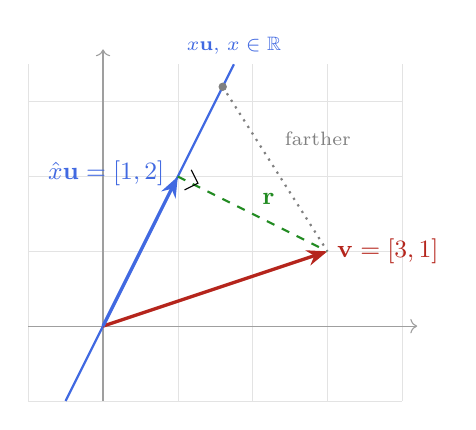
\begin{tikzpicture}[scale=0.95]
  \draw[step=1cm,gray!22,very thin] (-1,-1) grid (4,3.5);
  \draw[axisline] (-1,0) -- (4.2,0);
  \draw[axisline] (0,-1) -- (0,3.7);
  \draw[RoyalBlue,thick] (-0.5,-1) -- (1.75,3.5)
       node[above,font=\scriptsize]{$x\vc{u}$, $x\in\R$};
  \draw[vecarr,BrickRed] (0,0) -- (3,1);
  \node[right,font=\small,BrickRed] at (3,1) {$\vc{v}=[3,1]$};
  \draw[vecarr,RoyalBlue] (0,0) -- (1,2);
  \node[left,font=\small,RoyalBlue] at (0.95,2.05) {$\hat x\vc{u}=[1,2]$};
  \draw[dashed,thick,ForestGreen] (1,2) -- (3,1);
  \node[above right,font=\small,ForestGreen] at (2,1.5) {$\vc{r}$};
  \draw (1.0894,1.8211) -- (1.2683,1.9106) -- (1.1789,2.0894);
  \fill[gray] (1.6,3.2) circle (1.6pt);
  \draw[dotted,gray,thick] (1.6,3.2) -- (3,1);
  \node[right,font=\scriptsize,gray] at (2.3,2.5) {farther};
\end{tikzpicture}
\end{center}

\begin{ex}[The best constant]
\label{ex:mean}
Three measurements $\vc{v}=[\,1,2,2\,]$, and we want the single number $c$ that
best represents them. ``Best'' in the least-squares sense means minimizing
$\norm{\vc{v}-c\,\vc{u}}^{2}$ with $\vc{u}=[\,1,1,1\,]$, the sum of the squared
differences $(1-c)^{2}+(2-c)^{2}+(2-c)^{2}$. Then
$\hat c=\frac{1+2+2}{3}=\frac53$, the average. The mean of a list of numbers is
its least-squares constant.
\end{ex}

%==============================================================================
\section{The closest point in a column space}
%==============================================================================

%------------------------------------------------------------------------------
\subsection{The problem}
%------------------------------------------------------------------------------
Now let there be many unknowns. Let $\mt{A}\in\R^{m\times n}$ and
$\vc{b}\in\R^{m}$, typically with $m>n$ and $\vc{b}\notin\colsp{\mt{A}}$, so that
$\mt{A}\vc{x}=\vc{b}$ has no solution (\S45.1). For each $\vc{x}$ the
\textbf{residual} $\vc{r}=\vc{b}-\mt{A}\vc{x}$ measures how far the equations are
from holding.

\begin{defn}[Least-squares solution]
A \textbf{least-squares solution} of $\mt{A}\vc{x}=\vc{b}$ is a vector $\xh$ that
minimizes the length of the residual:
\[
  \xh\in\argmin_{\vc{x}\in\R^{n}}\ \norm{\mt{A}\vc{x}-\vc{b}}_2^{2}.
\]
\end{defn}

\noindent The name is literal. $\norm{\mt{A}\vc{x}-\vc{b}}^{2}$ is the sum of the
squares of the $m$ errors, one per equation, and we make that sum least. With
$n=1$ and $\mt{A}$ the single column $\vc{u}$, this is \S46 exactly.

%------------------------------------------------------------------------------
\subsection{The geometry}
%------------------------------------------------------------------------------
As $\vc{x}$ ranges over $\R^{n}$, the vector $\mt{A}\vc{x}$ ranges over the
column space (\S10.1). So the problem is: \emph{find the point of
$\colsp{\mt{A}}$ closest to $\vc{b}$.} In \S46 the subspace was a line, and the
closest point was the foot of the perpendicular. The same is true for any
subspace.

\begin{thm}
\label{thm:perp}
If $\xh$ makes the residual orthogonal to every column of $\mt{A}$, that is,
\[
  \mt{A}\T(\vc{b}-\mt{A}\xh)=\vc{0},
\]
then $\xh$ is a least-squares solution: $\norm{\mt{A}\vc{x}-\vc{b}}\ge\norm{\mt{A}\xh-\vc{b}}$
for every $\vc{x}$.
\end{thm}

\begin{proof}
Write $\vc{b}-\mt{A}\vc{x}=(\vc{b}-\mt{A}\xh)+\mt{A}(\xh-\vc{x})$. The second
piece is in $\colsp{\mt{A}}$, and the first is orthogonal to it:
\[
  \bigl(\mt{A}(\xh-\vc{x})\bigr)\T(\vc{b}-\mt{A}\xh)
  =(\xh-\vc{x})\T\,\mt{A}\T(\vc{b}-\mt{A}\xh)=(\xh-\vc{x})\T\vc{0}=0 .
\]
By the Pythagorean identity,
\[
  \norm{\vc{b}-\mt{A}\vc{x}}^{2}=\norm{\vc{b}-\mt{A}\xh}^{2}+\norm{\mt{A}(\xh-\vc{x})}^{2}
  \;\ge\;\norm{\vc{b}-\mt{A}\xh}^{2}.\qedhere
\]
\end{proof}

\noindent Why does the condition read $\mt{A}\T(\cdots)=\vc{0}$? A vector is
orthogonal to the whole column space exactly when it is orthogonal to each column
$\vc{a}_j$ (every vector of the column space is a combination of them). The
conditions $\vc{a}_j\T\vc{r}=0$, $j=1,\dots,n$, are the $n$ entries of
$\mt{A}\T\vc{r}$, because the rows of $\mt{A}\T$ are the columns of $\mt{A}$.

\begin{center}
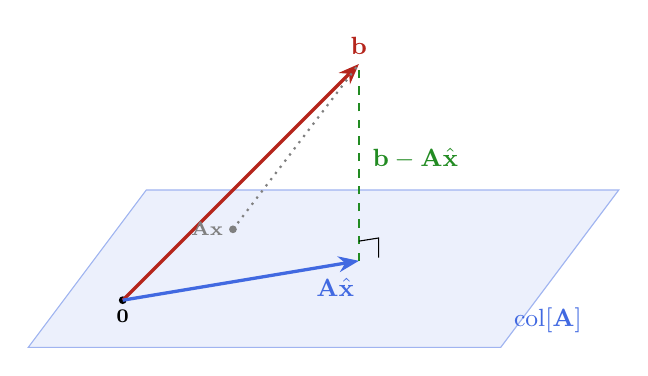
\begin{tikzpicture}[scale=1.0]
  % the plane col[A], drawn in perspective
  \fill[RoyalBlue!10] (0,0) -- (6,0) -- (7.5,2) -- (1.5,2) -- cycle;
  \draw[RoyalBlue!50] (0,0) -- (6,0) -- (7.5,2) -- (1.5,2) -- cycle;
  \node[font=\small,RoyalBlue] at (6.6,0.35) {$\colsp{\mt{A}}$};
  \coordinate (O) at (1.2,0.6);
  \coordinate (P) at (4.2,1.1);
  \coordinate (B) at (4.2,3.6);
  \coordinate (Q) at (2.6,1.5);
  \fill (O) circle (1.4pt) node[below,font=\scriptsize]{$\vc{0}$};
  \draw[vecarr,BrickRed] (O) -- (B);
  \node[above,font=\small,BrickRed] at (B) {$\vc{b}$};
  \draw[vecarr,RoyalBlue] (O) -- (P);
  \node[below,font=\small,RoyalBlue] at (3.9,1.0) {$\mt{A}\xh$};
  \draw[dashed,thick,ForestGreen] (P) -- (B);
  \node[right,font=\small,ForestGreen] at (4.25,2.4) {$\vc{b}-\mt{A}\xh$};
  \draw (4.2,1.35) -- (4.45,1.39) -- (4.45,1.14);
  \fill[gray] (Q) circle (1.4pt) node[left,font=\scriptsize,gray]{$\mt{A}\vc{x}$};
  \draw[dotted,thick,gray] (Q) -- (B);
\end{tikzpicture}
\end{center}

\noindent The residual of the best $\xh$ stands perpendicular to the column
space. Any other $\mt{A}\vc{x}$ in the plane is farther from $\vc{b}$, because the
dotted segment is the hypotenuse of a right triangle whose leg is the dashed one.

%------------------------------------------------------------------------------
\subsection{The normal equations}
%------------------------------------------------------------------------------
Multiply out the condition of Theorem~\ref{thm:perp}:
$\mt{A}\T\vc{b}-\mt{A}\T\mt{A}\xh=\vc{0}$.

\begin{defn}[Normal equations]
The \textbf{normal equations} of the system $\mt{A}\vc{x}=\vc{b}$ are
\[
  \boxed{\;\mt{A}\T\mt{A}\,\xh=\mt{A}\T\vc{b}.\;}
\]
\end{defn}

\noindent ``Normal'' is an old word for perpendicular: these equations say the
residual is normal to the column space. They form a \emph{square} system,
$n\times n$, even when $\mt{A}$ is tall and thin, and its matrix $\mt{A}\T\mt{A}$
is the one Part 6 studied. With $n=1$ and $\mt{A}=\vc{u}$, they read
$(\vc{u}\T\vc{u})\hat x=\vc{u}\T\vc{v}$, which is \S46.3.

%------------------------------------------------------------------------------
\subsection{The residual lives in the null space of \texorpdfstring{$\mt{A}\T$}{A'}}
%------------------------------------------------------------------------------
The condition $\mt{A}\T\vc{r}=\vc{0}$ says $\vc{r}\in\nullsp{\mt{A}\T}$. By
\S31.7 applied to $\mt{A}\T$, that null space is orthogonal to the row space of
$\mt{A}\T$, which is $\colsp{\mt{A}}$. So $\R^{m}$ splits into the column space
and the directions orthogonal to it, and least squares keeps the first piece of
$\vc{b}$ and discards the second. The map $\vc{b}\mapsto\mt{A}\xh$ is an
orthogonal projection, onto $\colsp{\mt{A}}$, and Part 10 writes down its
matrix.

%==============================================================================
\section{The same answer by calculus}
%==============================================================================

%------------------------------------------------------------------------------
\subsection{What we use}
%------------------------------------------------------------------------------
\lookback[the vector calculus unit] For a function $f:\R^{n}\to\R$, the partial
derivative $\partial f/\partial x_i$ differentiates in $x_i$ with the other
variables held fixed, and the \textbf{gradient} $\nabla f$ is the vector of all
$n$ of them (\S6--\S7 in two variables; \S11--\S12 in $n$). At a minimum of a
differentiable function, every partial derivative is zero, so $\nabla f=\vc{0}$.

%------------------------------------------------------------------------------
\subsection{The function}
%------------------------------------------------------------------------------
Expand $f(\vc{x})=\norm{\mt{A}\vc{x}-\vc{b}}^{2}$ as in \S46.2, using M6:
\[
  f(\vc{x})=(\mt{A}\vc{x}-\vc{b})\T(\mt{A}\vc{x}-\vc{b})
  =\vc{x}\T\mt{A}\T\mt{A}\vc{x}-\vc{x}\T\mt{A}\T\vc{b}-\vc{b}\T\mt{A}\vc{x}+\vc{b}\T\vc{b}.
\]
The two middle terms are $1\times1$ matrices, numbers, and each is the transpose
of the other, so they are equal:
\[
  f(\vc{x})=\vc{x}\T\mt{M}\vc{x}-2\,\vc{c}\T\vc{x}+\vc{b}\T\vc{b},
  \qquad \mt{M}=\mt{A}\T\mt{A},\quad \vc{c}=\mt{A}\T\vc{b}.
\]
A quadratic part, a linear part, and a constant.

%------------------------------------------------------------------------------
\subsection{Two gradients}
%------------------------------------------------------------------------------
\textbf{A linear function.} $g(\vc{x})=\vc{c}\T\vc{x}=c_1x_1+\cdots+c_nx_n$, so
$\partial g/\partial x_i=c_i$ and
\[
  \nabla(\vc{c}\T\vc{x})=\vc{c}.
\]
This is the $n$-variable version of $\frac{d}{dx}(cx)=c$.

\textbf{A quadratic function.} $h(\vc{x})=\vc{x}\T\mt{M}\vc{x}=\sum_{j}\sum_{k}m_{jk}x_jx_k$.
Differentiate in $x_i$. The terms containing $x_i$ are those with $j=i$ or $k=i$:
\[
  \frac{\partial h}{\partial x_i}
  =\sum_{k}m_{ik}x_k+\sum_{j}m_{ji}x_j
  =(\mt{M}\vc{x})_i+(\mt{M}\T\vc{x})_i .
\]
(The single term with $j=k=i$ is $m_{ii}x_i^{2}$, whose derivative $2m_{ii}x_i$ is
shared between the two sums.) So
\[
  \nabla(\vc{x}\T\mt{M}\vc{x})=(\mt{M}+\mt{M}\T)\,\vc{x}=2\mt{M}\vc{x}
  \quad\text{if }\mt{M}\text{ is symmetric,}
\]
the $n$-variable version of $\frac{d}{dx}(mx^{2})=2mx$.

\begin{ex}
$\mt{M}=\begin{bmatrix}2&1\\1&3\end{bmatrix}$: $h=2x_1^{2}+2x_1x_2+3x_2^{2}$, so
$\nabla h=[\,4x_1+2x_2,\ 2x_1+6x_2\,]$, which is $2\mt{M}\vc{x}$. \checkmark
\end{ex}

%------------------------------------------------------------------------------
\subsection{Setting the gradient to zero}
%------------------------------------------------------------------------------
$\mt{M}=\mt{A}\T\mt{A}$ is symmetric, so
\[
  \nabla f(\vc{x})=2\mt{A}\T\mt{A}\vc{x}-2\mt{A}\T\vc{b}.
\]
Setting $\nabla f=\vc{0}$ and dividing by $2$ gives
\[
  \mt{A}\T\mt{A}\,\xh=\mt{A}\T\vc{b},
\]
the normal equations again. Two routes, geometric and analytic, arrive at the
same square system.

%------------------------------------------------------------------------------
\subsection{A minimum, not a maximum}
%------------------------------------------------------------------------------
A zero gradient can also mark a maximum or a saddle. Here it cannot. Along any
line $\vc{x}+t\vc{d}$, $f$ is a one-variable quadratic in $t$ whose $t^{2}$
coefficient is
\[
  \vc{d}\T\mt{A}\T\mt{A}\vc{d}=\norm{\mt{A}\vc{d}}^{2}\ge0,
\]
so $f$ curves upward, or is flat, in every direction: its graph is a bowl.
Theorem~\ref{thm:perp} had already shown the critical point is a minimum. In
the language of the vector calculus unit (\S15), the Hessian of $f$ is the
constant matrix $2\mt{A}\T\mt{A}$, and $\vc{d}\T(2\mt{A}\T\mt{A})\vc{d}\ge0$ for
every $\vc{d}$.

%==============================================================================
\section{Solving the normal equations; fitting a line}
%==============================================================================

%------------------------------------------------------------------------------
\subsection{They always have a solution}
%------------------------------------------------------------------------------
A system with no solution has been replaced by another system. That only helps
if the new one is always solvable, and it is.

\begin{thm}
\label{thm:consistent}
For every $\mt{A}\in\R^{m\times n}$ and $\vc{b}\in\R^{m}$, the normal equations
$\mt{A}\T\mt{A}\vc{x}=\mt{A}\T\vc{b}$ have at least one solution.
\end{thm}

\begin{proof}
We need $\mt{A}\T\vc{b}\in\colsp{\mt{A}\T\mt{A}}$. Certainly
$\mt{A}\T\vc{b}\in\colsp{\mt{A}\T}$. Now
$\colsp{\mt{A}\T\mt{A}}\subseteq\colsp{\mt{A}\T}$, since
$\mt{A}\T\mt{A}\vc{x}=\mt{A}\T(\mt{A}\vc{x})$, and the two have the same
dimension: $\rank(\mt{A}\T\mt{A})=\rank(\mt{A})=\rank(\mt{A}\T)$ by \S33.2 and
\S33.3. A subspace inside another of the same dimension is all of it (extend its
basis, F2 and F3 of \S32.2). So $\colsp{\mt{A}\T\mt{A}}=\colsp{\mt{A}\T}$, which
contains $\mt{A}\T\vc{b}$.
\end{proof}

%------------------------------------------------------------------------------
\subsection{When the solution is unique}
%------------------------------------------------------------------------------
By \S31.6, the solutions of the normal equations form one solution plus
$\nullsp{\mt{A}\T\mt{A}}$, and $\nullsp{\mt{A}\T\mt{A}}=\nullsp{\mt{A}}$ (\S33.1).

\begin{thm}
\label{thm:unique}
The least-squares solution is unique if and only if $\mt{A}$ has full column
rank, i.e.\ its columns are independent.
\end{thm}

\noindent If the columns are dependent there are infinitely many least-squares
solutions. They all give the \emph{same} closest point $\mt{A}\xh$, since two of
them differ by a vector of $\nullsp{\mt{A}}$, which $\mt{A}$ sends to $\vc{0}$.
The point of the column space nearest $\vc{b}$ is always unique; only the recipe
$\xh$ for reaching it may not be.

%------------------------------------------------------------------------------
\subsection{How to solve them}
%------------------------------------------------------------------------------
The normal equations are an ordinary square system, so Part 8 solves them: form
$\mt{A}\T\mt{A}$ and $\mt{A}\T\vc{b}$, then eliminate and back substitute. With
full column rank the elimination finds $n$ pivots and a unique answer.

%------------------------------------------------------------------------------
\subsection{Fitting a line}
%------------------------------------------------------------------------------
\begin{ex}
\label{ex:fit}
The data of \S45.1: $(1,1)$, $(2,2)$, $(3,2)$. The model $y=c_0+c_1t$ gives one
equation per point, $\mt{A}\vc{x}=\vc{b}$ with
\[
  \mt{A}=\begin{bmatrix}1&1\\1&2\\1&3\end{bmatrix},\qquad
  \vc{x}=\begin{bmatrix}c_0\\c_1\end{bmatrix},\qquad
  \vc{b}=\begin{bmatrix}1\\2\\2\end{bmatrix},
\]
inconsistent by \S45.1. Form the normal equations:
\[
  \mt{A}\T\mt{A}=\begin{bmatrix}3&6\\6&14\end{bmatrix},\qquad
  \mt{A}\T\vc{b}=\begin{bmatrix}1+2+2\\1+4+6\end{bmatrix}=\begin{bmatrix}5\\11\end{bmatrix}.
\]
Eliminate:
$\begin{bmatrix}3&6&\vline&5\\6&14&\vline&11\end{bmatrix}\xrightarrow{R_2\gets R_2-2R_1}
\begin{bmatrix}3&6&\vline&5\\0&2&\vline&1\end{bmatrix}$, so $c_1=\frac12$ and
$c_0=\frac{5-6\cdot\frac12}{3}=\frac23$. The best line is
\[
  y=\tfrac23+\tfrac12t .
\]
Its predictions at $t=1,2,3$ are $\mt{A}\xh=[\,\frac76,\frac{10}{6},\frac{13}{6}\,]$,
and the residual is
\[
  \vc{r}=\vc{b}-\mt{A}\xh=\bigl[\,-\tfrac16,\ \tfrac13,\ -\tfrac16\,\bigr],
  \qquad
  \mt{A}\T\vc{r}=\bigl[\,-\tfrac16+\tfrac13-\tfrac16,\ \ -\tfrac16+\tfrac23-\tfrac12\,\bigr]=[\,0,0\,],
\]
orthogonal to both columns, as Theorem~\ref{thm:perp} requires. The sum of the
squared errors is $\frac1{36}+\frac4{36}+\frac1{36}=\frac16$, and no other line
does better.
\end{ex}

\begin{center}
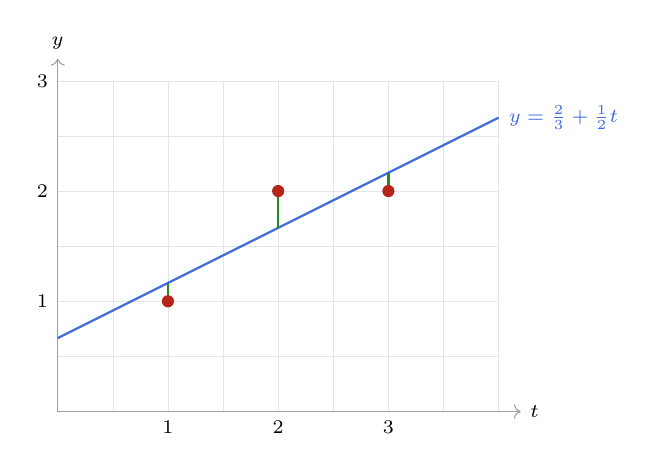
\begin{tikzpicture}[x=1.4cm,y=1.4cm]
  \draw[step=0.5,gray!20,very thin] (0,0) grid (4,3);
  \draw[axisline] (0,0) -- (4.2,0) node[right,font=\scriptsize,black]{$t$};
  \draw[axisline] (0,0) -- (0,3.2) node[above,font=\scriptsize,black]{$y$};
  \foreach \t in {1,2,3} \node[below,font=\scriptsize] at (\t,0) {$\t$};
  \foreach \y in {1,2,3} \node[left,font=\scriptsize] at (0,\y) {$\y$};
  \draw[RoyalBlue,thick] (0,0.6667) -- (4,2.6667)
       node[right,font=\scriptsize]{$y=\frac23+\frac12t$};
  \draw[ForestGreen,thick] (1,1) -- (1,1.1667);
  \draw[ForestGreen,thick] (2,2) -- (2,1.6667);
  \draw[ForestGreen,thick] (3,2) -- (3,2.1667);
  \fill[BrickRed] (1,1) circle (2.2pt);
  \fill[BrickRed] (2,2) circle (2.2pt);
  \fill[BrickRed] (3,2) circle (2.2pt);
\end{tikzpicture}
\end{center}

\noindent The green segments are the three entries of the residual. Least
squares makes the sum of their squares as small as possible.

%------------------------------------------------------------------------------
\subsection{Linear regression}
%------------------------------------------------------------------------------
In general, $m$ data points $(t_i,y_i)$ and the model $y=c_0+c_1t$ give the
$m\times2$ matrix with rows $[\,1,\ t_i\,]$. Its two columns, all ones and the
$t_i$, are independent unless every $t_i$ is the same, so by
Theorem~\ref{thm:unique} the best line is unique. This is \textbf{linear
regression}, the most used computation in statistics.

The method fits much more than lines. A parabola $y=c_0+c_1t+c_2t^{2}$ gives rows
$[\,1,\ t_i,\ t_i^{2}\,]$, and any model that is a combination of fixed functions
of $t$ with unknown coefficients works the same way. ``Linear'' refers to the
\emph{coefficients} $c_j$, which enter linearly, not to the shape of the curve.

%------------------------------------------------------------------------------
\subsection{Practice}
%------------------------------------------------------------------------------
\begin{enumerate}[label=\textbf{P\arabic*.},leftmargin=2.6em,itemsep=5pt]
  \item Find the multiple of $\vc{u}=[\,2,1,2\,]$ closest to $\vc{v}=[\,1,1,1\,]$,
        and check that the residual is orthogonal to $\vc{u}$.
  \item Fit the line $y=c_0+c_1t$ to the points $(0,6)$, $(1,0)$, $(2,0)$ by the
        normal equations, and check that the residual is orthogonal to both
        columns.
  \item What is the least-squares constant for the data $2,4,9$?
  \item Show that if $\vc{b}\in\colsp{\mt{A}}$, every least-squares solution
        solves $\mt{A}\vc{x}=\vc{b}$ exactly.
  \item Compute $\nabla(\vc{x}\T\mt{M}\vc{x})$ for the non-symmetric
        $\mt{M}=\begin{bmatrix}1&2\\0&3\end{bmatrix}$ directly, and compare with
        $(\mt{M}+\mt{M}\T)\vc{x}$.
  \item Write $\mt{A}$, $\mt{A}\T\mt{A}$ and $\mt{A}\T\vc{b}$ for fitting the
        parabola $y=c_0+c_1t+c_2t^{2}$ to $(-1,1)$, $(0,0)$, $(1,1)$, $(2,3)$.
\end{enumerate}

\subsubsection*{Answers}

\noindent\textbf{P1.} $\hat x=\frac{2+1+2}{4+1+4}=\frac59$; the closest point is
$\frac59[\,2,1,2\,]$, and the residual is $[\,-\frac19,\frac49,-\frac19\,]$, with
$-\frac29+\frac49-\frac29=0$. \checkmark

\smallskip
\noindent\textbf{P2.} $\mt{A}=\begin{bmatrix}1&0\\1&1\\1&2\end{bmatrix}$,
$\vc{b}=[\,6,0,0\,]$; $\mt{A}\T\mt{A}=\begin{bmatrix}3&3\\3&5\end{bmatrix}$,
$\mt{A}\T\vc{b}=[\,6,0\,]$. Elimination gives $2c_1=-6$, so $c_1=-3$ and $c_0=5$:
$y=5-3t$. Residual $[\,6-5,\ 0-2,\ 0+1\,]=[\,1,-2,1\,]$; its dot products with
$[\,1,1,1\,]$ and $[\,0,1,2\,]$ are $0$ and $0$. \checkmark

\smallskip
\noindent\textbf{P3.} The mean, $5$ (Example~\ref{ex:mean}).

\smallskip
\noindent\textbf{P4.} Some $\vc{x}_0$ has $\mt{A}\vc{x}_0=\vc{b}$, so the
smallest possible value of $\norm{\mt{A}\vc{x}-\vc{b}}$ is $0$. A least-squares
solution attains the smallest value, so $\norm{\mt{A}\xh-\vc{b}}=0$.

\smallskip
\noindent\textbf{P5.} $\vc{x}\T\mt{M}\vc{x}=x_1^{2}+2x_1x_2+3x_2^{2}$, with
gradient $[\,2x_1+2x_2,\ 2x_1+6x_2\,]$; and
$\mt{M}+\mt{M}\T=\begin{bmatrix}2&2\\2&6\end{bmatrix}$. They agree, and $2\mt{M}\vc{x}$
would be wrong, since $\mt{M}$ is not symmetric.

\smallskip
\noindent\textbf{P6.} $\mt{A}=\begin{bmatrix}1&-1&1\\1&0&0\\1&1&1\\1&2&4\end{bmatrix}$,
$\mt{A}\T\mt{A}=\begin{bmatrix}4&2&6\\2&6&8\\6&8&18\end{bmatrix}$,
$\mt{A}\T\vc{b}=[\,5,\ 6,\ 14\,]$ with $\vc{b}=[\,1,0,1,3\,]$.

\lookahead The normal equations were solved by elimination, because the matrix
inverse had not yet been defined in general. Part 10 defines it. Then the
least-squares solution has a formula, $\xh=(\mt{A}\T\mt{A})^{-1}\mt{A}\T\vc{b}$,
and the matrix in front of $\vc{b}$ becomes a generalized inverse in its own
right: the pseudo-inverse.

\end{document}
